\chapter{Objects}\label{ch:objects}

\hyphenation{cond-i-tion-al-ex-press-ion}
\hyphenation{con-se-quent-ex-press-ion}
\hyphenation{wide-spread}

\chapquotew{It was amazing to me, and it is still amazing, that people could not imagine what the psychological
difference would be to have an interactive terminal. You can talk about it on a blackboard until you are blue in the
face, and people would say, ``Oh, yes, but why do you need that?''$\ldots$ We used to try to think of all these
analogies, like describing it in terms of the difference between mailing a letter to your mother and getting on the
telephone. To this day I can still remember people only realizing when they saw a real demo, say, ``Hey, it talks back.
Wow! You just type that and you got an answer.''}{Fernando Corbat\'{o} (who worked on Whirlwind in the 1950s)\\Charles~Babbage~Institute interview, 1989}{11.8cm}%http://www.cbi.umn.edu/oh/pdf.phtml?id=92 Corbato interview


\begin{schemeregion}

So far, we have seen two main approaches for solving problems:
\begin{descriptionlist}
\item [\emph{Functional programming}] \forcenl Break a problem into a group of simpler procedures that can be composed to solve the problem (introduced in Chapter~\ref{ch:problems}).
\item [\emph{Data-centric programming}] \forcenl Model the data the problem involves, and develop procedures to manipulate that data (introduced in Chapter~\ref{ch:data}, and extended to imperative programming with mutation in the previous chapter).
\end{descriptionlist}

All computational problems involve both data and procedures.  All procedures act on some form of data; without data they can have no meaningful inputs and outputs.  Any data-focused design must involve some procedures to perform computations using that data.  

This chapter introduces a new problem-solving approach known as \definition{object-ori\-en\-ted programming}.  By packaging procedures and data together, object-or\-i\-en\-ted programming overcomes a weakness of both previous approaches: the data and the procedures that manipulate it are separate. 

Unlike many programming languages, Scheme does not provide special built-in support for objects.\footnote{This refers to the standard Scheme language, not the many extended Scheme languages provided by DrRacket.  The MzScheme language does provide additional constructs for supporting objects, but we do not cover them in this book.}  We build an object system ourselves, taking advantage of the stateful evaluation rules.  By building an object system from simple components, we provide a clearer and deeper understanding of how object systems work.  In Chapter~\ref{ch:interpreters}, we see how Python provides language support for object-oriented programming.

The next section introduces techniques for programming with objects that combine state with procedures that manipulate that state.  Section~\ref{sec:inheritance} describes \definition{inheritance}, a powerful technique for programming with objects by implementing new objects that add or modify the behaviors of previously implemented objects.  Section~\ref{sec:oohistory} provides some historical background on the development of object-oriented programming.

\section{Packaging Procedures and State}

Recall our counter from Example~\ref{example:counter}:\index{general}{counter}
\begin{schemedisplay}
(define (update-counter!) (set! counter (+ counter 1)) counter)
\end{schemedisplay}
%The \scheme|update-counter!| procedure increments the value of the \scheme|counter| variable, which is stored in the global environment, and evaluates to the resulting counter value.  
Every time an application of \scheme|update-counter!| is evaluated, we expect to obtain a value one larger than the previous application.  This only works, however, if there are no other evaluations that modify the \scheme|counter| variable.  Hence, we can only have one counter: there is only one \scheme|counter| place in the global environment.  If we want to have a second counter, we would need to define a new variable (such as \scheme|counter2|, and implement a new procedure, \scheme|update-counter2!|, that is identical to \scheme|update-counter!|, but manipulates \scheme|counter2| instead.  For each new counter, we would need a new variable and a new procedure.

\subsection{Encapsulation}\label{sec:encapsulation}\index{general}{encapsulation}

It would be more useful to package the counter variable with the procedure that manipulates it.  Then we could create as many counters as we want, each with its own counter variable to manipulate.  

The Stateful Application Rule (from Section~\ref{sec:state-rules}) suggests a way to do this: evaluating an application creates a new environment, so a counter variable defined an the application environment is only visible through body of the created procedure.  

The \scheme|make-counter| procedure creates a counter object that packages the \scheme|count| variable with the procedure that increases its value:
\begin{schemedisplay}
(define (make-counter)
  ((lambda (count) 
     (lambda () (set! count (+ 1 count)) count))
   0))
\end{schemedisplay}

Each application of \scheme|make-counter| produces a new object that is a procedure with its own associated \scheme|count| variable.  Protecting state so it can only be manipulated in controlled ways is known as \definition{encapsulation}.  

The \scheme|count| place is encapsulated within the counter object.  Whereas the previous counter used the global environment to store the counter in a way that could be manipulated by other expressions, this version encapsulates the counter variable so the only way to manipulate the counter value is through the counter object. 

An equivalent \scheme|make-counter| definition uses a let expression to make the initialization of the \scheme|count| variable clearer:

\begin{schemedisplay}
(define (make-counter)
  (let ((count 0))
    (lambda () (set! count (+ 1 count)) count)))
\end{schemedisplay}

Figure~\ref{fig:make-counter} depicts the environment after creating two counter objects and applying one of them.

\begin{figure}[bth]
\begin{center}
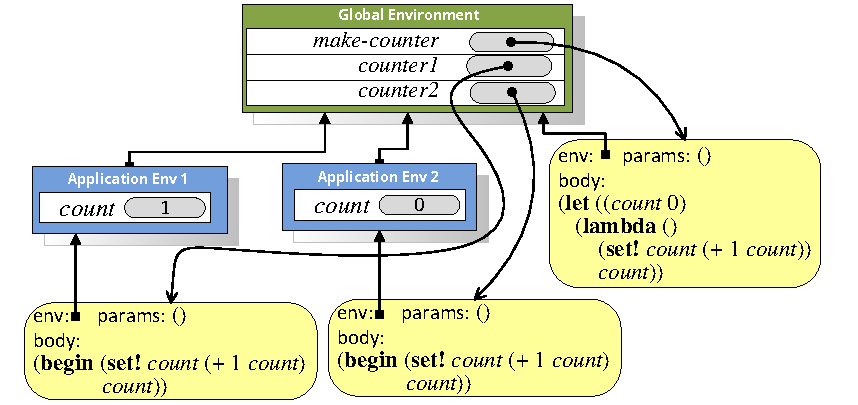
\includegraphics[width=5.0in]{figures/make-counter.pdf}
\caption{Environment produced by evaluating:}\label{fig:make-counter}
\vspace{-1.5ex}
\begin{schemedisplay}
(define counter1 (make-counter)) 
(define counter2 (make-counter)) 
(counter1)
\end{schemedisplay}
%({\bf define} \var{counter1} (\var{make-counter})) ({\bf define} \var{counter2} (\var{make-counter})) (\var{counter1}).}\label{fig:make-counter}
\end{center}
\end{figure}
 
\subsection{Messages}\label{sec:messages}\index{general}{messages}

The object produced by \scheme|make-counter| is limited to only one behavior: every time it is applied the associated count variable is increased by one and the new value is output.  To produce more useful objects, we need a way to combine state with multiple behaviors.  

For example, we might want a counter that can also return the current count and reset the count.  We do this by adding a \scheme|message| parameter to the procedure produced by \scheme|make-counter|:

\begin{schemedisplay}
(define (make-counter)
  (let ((count 0))
    (lambda (message)
      (if (eq? message 'get-count) count
          (if (eq? message 'reset!) (set! count 0)
              (if (eq? message 'next!) (set! count (+ 1 count))              
                  (error "Unrecognized message")))))))
\end{schemedisplay}

Like the earlier \scheme|make-counter|, this procedure produces a procedure with an environment containing a frame with a place named \scheme|count|.  The produced procedure takes a \scheme|message| parameter and selects different behavior depending on the input message.  

The \scheme|message| parameter is a Symbol.  A Symbol is a sequence of characters preceded by a quote character such as \scheme|'next!|.  Two Symbols are equal, as determined by the \scheme|eq?| procedure, if their sequences of characters are identical.  The running time of the \scheme|eq?| procedure on symbol type inputs is constant; it does not increase with the length of the symbols since the symbols can be represented internally as small numbers and compared quickly using number equality.  This makes symbols a more efficient way of selecting object behaviors than Strings, and a more memorable way to select behaviors than using Numbers.\index{general}{symbol}

Here are some sample interactions using the counter object:
\begin{code}
\scheme|> (define counter (make-counter))|\\
\scheme|> (counter 'next!)|\\
\scheme|> (counter 'get-count)|\\
\schemeresult|1|\\
\scheme|> (counter 'previous!)|\\
 \bugresult{Unrecognized message}
\end{code}

\shortsection{Conditional expressions}\index{general}{conditional expression}\index{general}{cond}  For objects with many behaviors, the nested if expressions can get quite cumbersome.  Scheme provides a compact conditional expression for combining many if expressions into one smaller expression:  
\begin{bnfgrammarm}{CondClauseList}
\bnfrule{Expression}{\nonterminal{CondExpression}}
\bnfrule{CondExpression}{\scheme|(cond \CondClauseList)|}
\bnfrule{CondClauseList}{\nonterminal{CondClause} \nonterminal{CondClauseList}}
\bnfrule{CondClauseList}{$\epsilon$}
\bnfrule{CondClause}{\scheme|(\ExpressionP \ExpressionV)|}
\end{bnfgrammarm}

\cut{The evaluation rule for a conditional expression is:

\mevalrule{Evaluation Rule 9: Conditional}{A conditional expression of the form, \scheme|(cond)| has no value.  To evaluate a conditional expression of the form,
\begin{schemedisplay}
(cond (\ExpressionPA \ExpressionVA)
      (\ExpressionPB \ExpressionVB)
      \cdots
      (\ExpressionPK \ExpressionVK))
\end{schemedisplay}
in the current execution environment, $E$, first evaluate \nonterminal{Expression$_{p1}$} in $E$.  If it evaluates to \schemeresult|true|, the value of the conditional expression is the value of \nonterminal{Expression$_{c1}$} in $E$.  Otherwise, the value of the conditional expression is the value in $E$ of the conditional expression,
\begin{schemedisplay}
(cond (\ExpressionPB \ExpressionVB)
      \cdots
      (\ExpressionPK \ExpressionVK))
\end{schemedisplay}
}
}
%The evaluation rule is defined recursively.  It continues through the predicate expressions until finding the first predicate that evaluates to \scheme|true|.  The value of the conditional expression is the value of the consequent expression associated with the first true predicate.  If all the predicate expressions evaluate to \scheme|false|, the conditional expression has no value.

The evaluation rule for a conditional expression can be defined as a transformation into an if expression:
\mevalrule{Evaluation Rule 9: Conditional}{The conditional expression \scheme|(cond)| has no value.  All other conditional expressions are of the form \scheme|(cond (\ExpressionPA \ExpressionVA) \Rest)| where \scheme|\Rest| is a list of conditional clauses.  The value of such a conditional expression is the value of the if expression:
\begin{schemedisplay}
(if \ExpressionPA \ExpressionVA (cond \Rest))
\end{schemedisplay}
}

This evaluation rule is recursive since the transformed expression still includes a conditional expression, but uses the empty conditional with no value as its base case.

The conditional expression can be used to define \scheme|make-counter| more clearly than the nested if expressions:
\begin{schemedisplay}
(define (make-counter)
  (let ((count 0))
    (lambda (message)
      (cond ((eq? message 'get-count) count)
            ((eq? message 'reset!)    (set! count 0))
            ((eq? message 'next!)     (set! count (+ 1 count)))            
            (true (error "Unrecognized message"))))))
\end{schemedisplay}

\index{general}{else}For linguistic convenience, Scheme provides a special syntax \scheme|else| for use in conditional expressions.  When used as the predicate in the last conditional clause it means the same thing as \scheme|true|.  So, we could write the last clause equivalently as \scheme|(else (error "Unrecognized message"))|.

\shortsection{Sending messages}  A more natural way to interact with objects is to define a generic procedure that takes an object and a message as its parameters, and send the message to the object. 

The \scheme|ask| procedure is a simple procedure that does this:
\begin{schemedisplay}
(define (ask object message) (object message))
\end{schemedisplay}

It applies the \scheme|object| input to the \scheme|message| input.  So, \scheme|(ask counter 'next!)| is equivalent to \scheme|(counter 'next!)|, but looks more like passing a message to an object than applying a procedure.  Later, we will develop more complex versions of the \scheme|ask| procedure to provide a more powerful object model.

\shortsection{Messages with parameters} Sometimes it is useful to have behaviors that take additional parameters.  For example, we may want to support a message \scheme|adjust!| that increases the counter value by an input value.  

To support such behaviors, we generalize the behaviors so that the result of applying the message dispatching procedure is itself a procedure.  The procedures for \scheme|reset!|, \scheme|next!|, and \scheme|get-count| take no parameters; the procedure for \scheme|adjust!| takes one parameter.

\begin{schemedisplay}
(define (make-adjustable-counter)
  (let ((count 0))
    (lambda (message)
      (cond ((eq? message 'get-count) (lambda () count))
            ((eq? message 'reset!) (lambda () (set! count 0)))
            ((eq? message 'next!) (lambda () (set! count (+ 1 count))))            
            ((eq? message 'adjust!) 
             (lambda (val) (set! count (+ count val))))
            (else (error "Unrecognized message"))))))
\end{schemedisplay}

We also need to also change the \scheme|ask| procedure to pass in the extra arguments.  So far, all the procedures we have defined take a fixed number of operands.  To allow \scheme|ask| to work for procedures that take a variable number of arguments, we use a special definition construct:\index{general}{definition}

\begin{bnfgrammarm}{Definition}
\bnfrule{Definition}{\scheme|(define (|\terminal{\emph{Name}} \nonterminal{Parameters} \terminal{.} \nonterminal{Name$_{Rest}$}\scheme|)| \nonterminal{Expression}\scheme|)|}
\end{bnfgrammarm}

The name following the dot is bound to all the remaining operands combined into a list.  This means the defined procedure can be applied to $n$ or more operands where $n$ is the number of names in \nonterminal{Parameters}.  If there are only $n$ operand expressions, the value bound to \nonterminal{Name$_{Rest}$} is \schemeresult{null}.  If there are $n+k$ operand expressions, the value bound to \nonterminal{Name$_{Rest}$} is a list containing the values of the last $k$ operand expressions.

\index{general}{apply}To apply the procedure we use the built-in \scheme|apply| procedure which takes two inputs, a Procedure and a List.  It applies the procedure to the values in the list, extracting them from the list as each operand in order.  
\begin{schemedisplay}
(define (ask object message . args)
  (apply (object message) args))
\end{schemedisplay}

We can use the new \scheme|ask| procedure with two or more parameters to invoke methods with any number of arguments (e.g., \scheme|> (define counter (make-adjustable-counter)) (ask counter 'adjust! 5)|).

%\begin{code}
%\scheme|> (define counter (make-adjustable-counter))|\\
%\scheme|> (ask counter 'next!)|\\
%\scheme|> (ask counter 'get-count)|\\
%\schemeresult|6|
%\end{code}

\subsection{Object Terminology}\label{sec:objectterminology}

An \definition{object} is an entity that packages state and procedures.  

The state variables that are part of an object are called \definition{instance variables}.  The instance variables are stored in places that are part of the application environment for the object.  This means they are encapsulated with the object and can only be accessed through the object.  An object produced by \scheme|(make-counter)| defines a single instance variable, \scheme|count|.

The procedures that are part of an object are called \definition{methods}. Methods may provide information about the state of an object (we call these \emph{observers}) or modify the state of an object (we call these \emph{mutators}).  An object produced by \scheme|(make-counter)| provides three methods: \scheme|reset!| (a mutator), \scheme|next!| (a mutator), and \scheme|get-count| (an observer).  

An object is manipulated using the object's methods. We \definition{invoke} a method on an object by sending the object a message.  This is analogous to applying a procedure.  

A \definition{class} is a kind of object.  Classes are similar to data types.  They define a set of possible values and operations (methods in the object terminology) for manipulating those values.  
We also need procedures for creating new objects, such as the \scheme|make-counter| procedure above. We call these \definition{constructors}.  By convention, we call the constructor for a class \scheme|make-<class>| where \scheme|<class>| is the name of the class.  Hence, an instance of the \scheme|counter| class is the result produced when the \scheme|make-counter| procedure is applied.

\beforeex
\begin{exercise}
Modify the \scheme|make-counter| definition to add a \scheme|previous!| method that decrements the counter value by one.
\solution{\LATER{}}
\end{exercise}
\afterex

\beforesplitex
\begin{exercise}
\goldstar\label{exercise:varcounter}
Define a \scheme|variable-counter| object that provides these methods:
\begin{descriptionlist}
\item[\scheme|make-variable-counter|: Number $\rightarrow$ VariableCounter]\forcenl Creates a \scheme|variable-counter| object with an initial counter value of \snumber{0} and an initial increment value given by the parameter.
\item[\scheme|set-increment!|: Number $\rightarrow$ Void]\forcenl Sets the increment amount for this counter to the input value.
\item[\scheme|next!|: Void $\rightarrow$ Void] \forcenl Adds the increment amount to the value of the counter.
\item[\scheme|get-count|: Void $\rightarrow$ Number ] \forcenl Outputs the current value of the counter.
\end{descriptionlist}
Here are some sample interactions using a \scheme|variable-counter| object:
\begin{code}
\scheme|> (define vcounter (make-variable-counter 1))|\\
\scheme|> (ask vcounter 'next!)|\\
\scheme|> (ask vcounter 'set-increment! 2)|\\
\scheme|> (ask vcounter 'next!)|\\
\scheme|> (ask vcounter 'get-count)|\\
\schemeresult|3|
\end{code}
\solution{\LATER{}}
\end{exercise}
\aftersplitex
%\marginquote{I invented the term ``Object-Oriented'' and I can tell you I did not have C++ in mind.}{Alan Kay}

\section{Inheritance}\label{sec:inheritance}

Objects are particularly well-suited to programs that involve modeling real or imaginary worlds such as graphical user interfaces (modeling windows, files, and folders on a desktop), simulations (modeling physical objects in the real world and their interactions), and games (modeling creatures and things in an imagined world).  

Objects in the real world (or most simulated worlds) are complex.  Suppose we are implementing a game that simulates a typical university.  It might include many different kinds of objects including places (which are stationary and may contain other objects), things, and people.  There are many different kinds of people, such as students and professors.  All objects in our game have a name and a location; some objects also have methods for talking and moving.  We could define classes independently for all of the object types, but this would involve a lot of duplicate effort.  It would also make it hard to add a new behavior to all of the objects in the game without modifying many different procedures.  

The solution is to define more specialized kinds of objects using the definitions of other objects.  For example, a \scheme|student| is a kind of \scheme|person|.\cut{, which is a kind of \scheme|movable-object|, which is a kind of \scheme|sim-object| (simulation object).} A \scheme|student| has all the behaviors of a normal \scheme|person|, as well as some behaviors particular to a \scheme|student| such as choosing a major and graduating.  To implement a \scheme|student| class, we want to reuse methods from the \scheme|person| class without needing to duplicate them in the \scheme|student| implementation.  We call the more specialized class (in this case the \scheme|student| class) the \definition{subclass} and say \scheme|student| is a subclass of \scheme|person|.  The reused class is known as the \definition{superclass}, so \scheme|person| is the superclass of \scheme|student|.  A class can have many subclasses but only one superclass.\footnote{Some object systems (such as the one provided by the C++ programming language) allow a class to have more than one superclass.  This can be confusing, though.  If a class has two superclasses and both define methods with the same name, it may be ambiguous which of the methods is used when it is invoked on an object of the subclass.  In our object system, a class may have only one superclass.}  

Figure~\ref{fig-inheritance} illustrates some inheritance relationships for a university simulator.  The arrows point from subclasses to their superclass.  A class may be both a subclass to another class, and a superclass to a different class.  For example, \scheme|person| is a subclass of \scheme|movable-object|, but a superclass of \scheme|student| and \scheme|professor|.  

\begin{figure}[bth]
\begin{center}
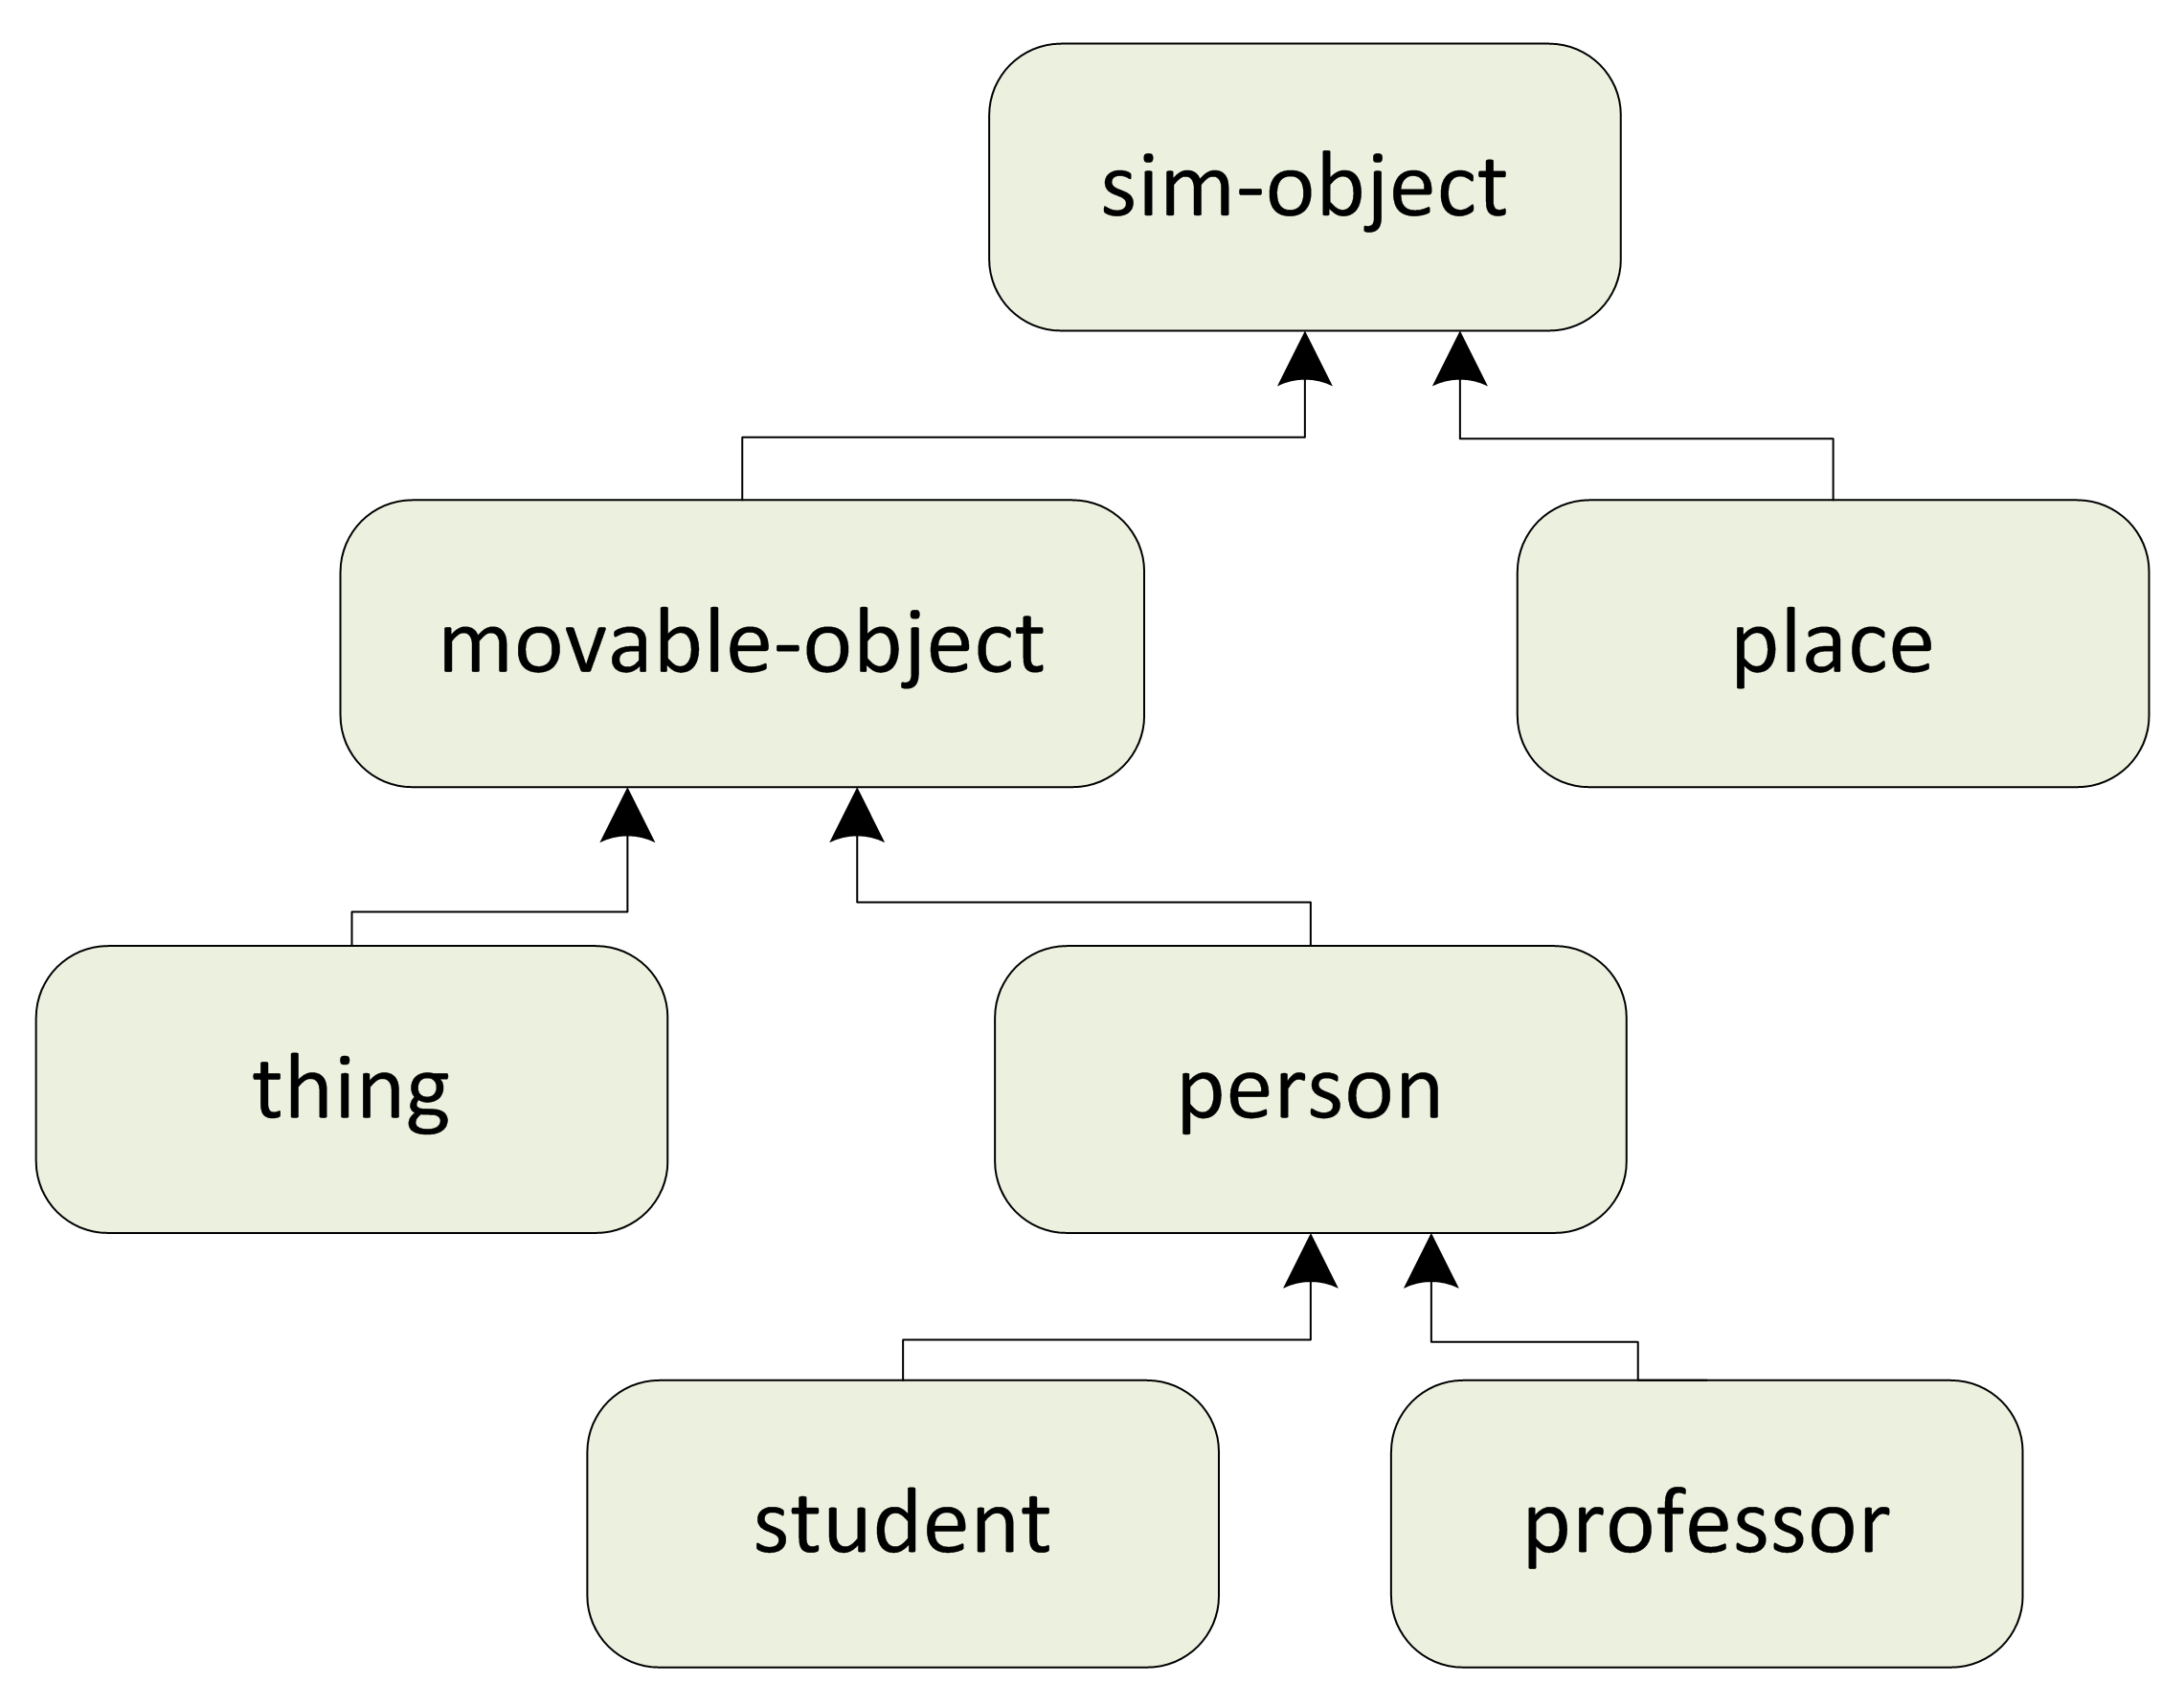
\includegraphics[width=2.2in]{figures/inheritance.png}
\caption{Inheritance hierarchy.}\label{fig-inheritance}
\end{center}
\end{figure}

Our goal is to be able to reuse superclass methods in subclasses.  When a method is invoked in a subclass, if the subclass does not provide a definition of the method, then the definition of the method in the superclass is used.  This can continue up the superclass chain.  For instance, \scheme|student| is a subclass of \scheme|person|, which is a subclass of \scheme|movable-object|, which is a subclass of \scheme|sim-object| (simulation object), which is the superclass of all classes in the simulator.  

Hence, if the \scheme|sim-object| class defines a \scheme|get-name| method, when the \scheme|get-name| method is invoked on a \scheme|student| object, the implementation of \scheme|get-name| in the \scheme|sim-object| class will be used (as long as neither \scheme|person| nor \scheme|movable-object| defines its own \scheme|get-name| method).  

When one class implementation uses the methods from another class we say the subclass \definition{inherits} from the superclass.  Inheritance is a powerful way to obtain many different objects with a small amount of code.  

\subsection{Implementing Subclasses} 

To implement inheritance we change class definitions so that if a requested method is not defined by the subclass, the method defined by its superclass will be used. 

The \scheme|make-sub-object| procedure does this.  It takes two inputs, a superclass object and the object dispatching procedure of the subclass, and produces an instance of the subclass which is a procedure that takes a message as input and outputs the method corresponding to that message.  If the method is defined by the subclass, the result will be the subclass method.  If the method is not defined by the subclass, it will be the superclass method.

\begin{schemedisplay}
(define (make-sub-object super subproc)
  (lambda (message)
    (let ((method (subproc message)))
      (if method method (super message)))))
\end{schemedisplay}

When an object produced by \scheme|(make-sub-object obj proc)| is applied to a message, it first applies the subclass dispatch procedure to the message to find an appropriate method if one is defined.  If no method is defined by the subclass implementation, it evaluates to \scheme|(super message)|, the method associated with the \scheme|message| in the superclass.

\shortsection{References to self} It is useful to add an extra parameter to all methods so the object on which the method was invoked is visible.  Otherwise, the object will lose its special behaviors as it is moves up the superclasses.  We call this the \scheme|self| object (in some languages it is called the \emph{this} object instead).  To support this, we modify the \scheme|ask| procedure to pass in the object parameter to the method:
\begin{schemedisplay}
(define (ask object message . args)
  (apply (object message) object args))
\end{schemedisplay}

All methods now take the \scheme|self| object as their first parameter, and may take additional parameters.  So, the \scheme|counter| constructor is defined as:
\begin{schemedisplay}
(define (make-counter)
  (let ((count 0))
    (lambda (message)
      (cond 
       ((eq? message 'get-count) (lambda (self) count))           
       ((eq? message 'reset!) (lambda (self) (set! count 0)))
       ((eq? message 'next!) (lambda (self) (set! count (+ 1 count))))           
       (else (error "Unrecognized message"))))))
\end{schemedisplay}          

\shortsection{Subclassing counter} Since subclass objects cannot see the instance variables of their superclass objects directly, if we want to provide a versatile counter class we need to also provide a \scheme|set-count!| method for setting the value of the counter to an arbitrary value.  For reasons that will become clear later, we should use \scheme|set-count!| everywhere the value of the \scheme|count| variable is changed instead of setting it directly:
\begin{schemedisplay}
(define (make-counter)
  (let ((count 0))
    (lambda (message)
      (cond 
       ((eq? message 'get-count) (lambda (self) count))
       ((eq? message 'set-count!) (lambda (self val) (set! count val)))       
       ((eq? message 'reset!) (lambda (self) (ask self 'set-count! 0)))
       ((eq? message 'next!)   
        (lambda (self) (ask self 'set-count! (+ 1 (ask self 'current)))))
       (else (error "Unrecognized message"))))))
\end{schemedisplay}          

Previously, we defined \scheme|make-adjustable-counter| by repeating all the code from \scheme|make-counter| and adding an \scheme|adjust!| method.  With inheritance, we can define \scheme|make-adjustable-counter| as a subclass of \scheme|make-counter| without repeating any code:

\begin{schemedisplay}
(define (make-adjustable-counter)
  (make-sub-object
   (make-counter)
   (lambda (message)
     (cond 
      ((eq? message 'adjust!) 
       (lambda (self val) 
         (ask self 'set-count! (+ (ask self 'get-count) val))))
       (else false)))))
\end{schemedisplay}          

We use \scheme|make-sub-object| to create an object that inherits the behaviors from one class, and extends those behaviors by defining new methods in the subclass implementation.  

The new \scheme|adjust!| method takes one Number parameter (in addition to the \scheme|self| object that is passed to every method) and adds that number to the current counter value.  It cannot use \scheme|(set! count (+ count val))| directly, though, since the \scheme|count| variable is defined in the application environment of its superclass object and is not visible within \scheme|adjustable-counter|.  Hence, it accesses the counter using the \scheme|set-count!| and \scheme|get-count| methods provided by the superclass.

Suppose we create an \scheme|adjustable-counter| object:
\begin{schemedisplay}
(define acounter (make-adjustable-counter))
\end{schemedisplay}
Consider what happens when \scheme|(ask acounter 'adjust! 3)| is evaluated.  The \scheme|acounter| object is the result of the application of \scheme|make-sub-object| which is the procedure,
\begin{schemedisplay}
(lambda (message)
  (let ((method (subproc message)))
    (if method method (super message)))))
\end{schemedisplay}
where \scheme|super| is the \scheme|counter| object resulting from evaluating \scheme|(make-counter)| and \scheme|subproc| is the procedure created by the lambda expression in \scheme|make-adjustable-counter|.  The body of \scheme|ask| evaluates \scheme|(object message)| to find the method associated with the input message, in this case \scheme|'adjust!|.  The \scheme|acounter| object takes the \scheme|message| input and evaluates the let expression: 
\begin{schemedisplay}
(let ((method (subproc message))) \ldots)
\end{schemedisplay}  
The result of applying \scheme|subproc| to \scheme|message| is the \scheme|adjust!| procedure defined by \scheme|make-adjustable-counter|: 
\begin{schemedisplay}
(lambda (self val) 
  (ask self 'set-count! (+ (ask self 'get-count) val)))
\end{schemedisplay}
Since this is not \schemeresult|false|, the predicate of the if expression is non-false and the value of the consequent expression, \scheme|method|, is the result of the procedure application.  The \scheme|ask| procedure uses \scheme|apply| to apply this procedure to the \scheme|object| and \scheme|args| parameters.  The \scheme|object| is the \scheme|acounter| object, and the \scheme|args| is the list of the extra parameters, in this case \scheme|(3)|.

Thus, the \scheme|adjust!| method is applied to the \scheme|acounter| object and \scheme|3|.  The body of the \scheme|adjust!| method uses \scheme|ask| to invoke the \scheme|set-count!| method on the \scheme|self| object.  As with the first invocation, the body of \scheme|ask| evaluates \scheme|(object message)| to find the method.  In this case, the subclass implementation provides no \scheme|set-count!| method so the result of \scheme|(subproc message)| in the application of the subclass object is \schemeresult|false|.  Hence, the alternate expression is evaluated: \scheme|(super message)|.  This evaluates to the method associated with the \scheme|set-count!| message in the superclass.  The \scheme|ask| body will apply this method to the \scheme|self| object, setting the value of the counter to the new value.

We can define new classes by defining subclasses of previously defined classes.  For example, \scheme|reversible-counter| inherits from \scheme|adjustable-counter|:
\begin{schemedisplay}
(define (make-reversible-counter)
  (make-subobject
   (make-adjustable-counter)
   (lambda (message)
     (cond 
      ((eq? message 'previous!) (lambda (self) (ask self 'adjust! -1)))
      (else false)))))	
\end{schemedisplay}

The \scheme|reversible-counter| object defines the \scheme|previous!| method which provides a new behavior.  If the message to a \scheme|adjustable-counter| object is not \scheme|previous!|, the method from its superclass, \scheme|adjustable-counter| is used.  Within the \scheme|previous!| method we use \scheme|ask| to invoke the \scheme|adjust!| method on the \scheme|self| object.  Since the subclass implementation does not provide an \scheme|adjust!| method, this results in the superclass method being applied.

\subsection{Overriding Methods}\label{sec:overriding}
In addition to adding new methods, subclasses can replace the definitions of methods defined in the superclass. When a subclass replaces a method defined by its superclass, then the subclass method \indexeddefinition{overrides}{override} the superclass method.  When the method is invoked on a subclass object, the new method will be used.

For example, we can define a subclass of \scheme|reversible-counter| that is not allowed to have negative counter values.  If the counter would reach a negative number, instead of setting the counter to the new value, it produces an error message and maintains the counter at zero.  We do this by overriding the \scheme|set-count!| method, replacing the superclass implementation of the method with a new implementation.

\begin{schemedisplay}
(define (make-positive-counter)
  (make-subobject
   (make-reversible-counter)
   (lambda (message)
     (cond 
      ((eq? message 'set-count!)
       (lambda (self val) (if (< val 0) (error "Negative count") 
                                        \ldots)))
      (else false)))))
\end{schemedisplay}
What should go in place of the $\ldots$?  When the value to set the count to is not negative, what should happen is the count is set as it would be by the superclass \scheme|set-count!| method.  In the \scheme|positive-counter| code though, there is no way to access the \scheme|count| variable since it is in the superclass procedure's application environment.  There is also no way to invoke the superclass' \scheme|set-count!| method since it has been overridden by \scheme|positive-counter|.

The solution is to provide a way for the subclass object to obtain its superclass object.  We can do this by adding a \scheme|get-super| method to the object produced by \scheme|make-sub-object|:
\begin{schemedisplay}
(define (make-sub-object super subproc)
  (lambda (message)
    (if (eq? message 'get-super) 
        (lambda (self) super)
        (let ((method (subproc message)))            
          (if method method (super message))))))
\end{schemedisplay}
Thus, when an object produced by \scheme|make-sub-object| is passed the \scheme|get-super| message it returns a method that produces the \scheme|super| object.  The rest of the procedure is the same as before, so for every other message it behaves like the earlier \scheme|make-sub-object| procedure.

With the \scheme|get-super| method we can define the \scheme|set-count!| method for \scheme|positive-counter|, replacing the $\ldots$ with:
\begin{schemedisplay}
(ask (ask self 'get-super) 'set-count! val))
\end{schemedisplay}

Figure~\ref{fig:counter-hierarchy} shows the subclasses that inherit from \scheme|counter| and the methods they define or override.  

\begin{figure}[bthp]
\begin{center}
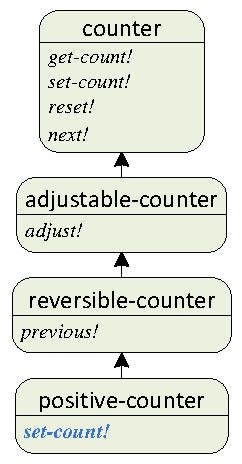
\includegraphics[width=1.2in]{figures/counter-hierarchy.pdf}
\caption{Counter class hierarchy.}\label{fig:counter-hierarchy}
\end{center}
\end{figure}

\groupcontent{
Consider these sample interactions with a \scheme|positive-counter| object:
\begin{code}
\scheme|> (define poscount (make-positive-counter))|\\
\scheme|> (ask poscount 'next!)|\\
\scheme|> (ask poscount 'previous!)|\\
\scheme|> (ask poscount 'previous!)|\\
\bugresult{Negative count}\\
\scheme|> (ask poscount 'get-count)|\\
\schemeresult|0|
\end{code}}

For the first \scheme|ask| application, the \scheme|next!| method is invoked on a \scheme|positive-counter| object.  Since the \scheme|positive-counter| class does not define a \scheme|next!| method, the message is sent to the superclass, \scheme|reversible-counter|.  The \scheme|reversible-counter| implementation also does not define a \scheme|next!| method, so the message is passed up to its superclass, \scheme|adjustable-counter|.  This class also does not define a \scheme|next!| method, so the message is passed up to its superclass, \scheme|counter|.  The \scheme|counter| class defines a \scheme{next!} method, so that method is used.

For the next \scheme|ask|, the \scheme|previous!| method is invoked.  Since the \scheme|positive-counter| class does not define a \scheme|previous!| method, the message is sent to the superclass.  The superclass, \scheme|reversible-counter|, defines a \scheme|previous!| method.  Its implementation involves an invocation of the \scheme|adjust!| method: \scheme|(ask self 'adjust! -1)|.  This invocation is done on the \scheme|self| object, which is an instance of the \scheme|positive-counter| class.  Hence, the \scheme|adjust!| method is found from the \scheme|positive-counter| class implementation.  This is the method that overrides the \scheme|adjust!| method defined by the \scheme|adjustable-counter| class.  Hence, the second invocation of \scheme|previous!| produces the ``Negative count'' error and does not adjust the count to \schemeresult|-1|.  

The property this object system has where the method invoked depends on the object is known as \definition{dynamic dispatch}.  The method used for an invocation depends on the \scheme|self| object.  In this case, for example, it means that when we inspect the implementation of the \scheme|previous!| method in the \scheme|reversible-counter| class by itself it is not possible to determine what procedure will be applied for the method invocation, \scheme|(ask self 'adjust! -1)|.  It depends on the actual \scheme|self| object: if it is a \scheme|positive-counter| object, the \scheme|adjust!| method defined by \scheme|positive-counter| is used; if it is a \scheme|reversible-counter| object, the \scheme|adjust!| method defined by \scheme|adjustable-counter| class (the superclass of \scheme|reversible-counter|) is used.  

Dynamic dispatch provides for a great deal of expressiveness.  It enables us to use the same code to produce many different behaviors by overriding methods in subclasses.  This is very useful, but also very dangerous --- it makes it impossible to reason about what a given procedure does, without knowing about all possible subclasses.  For example, we cannot make any claims about what the \scheme|previous!| method in \scheme|reversible-counter| actually does without knowing what the \scheme|adjust!| method does in all subclasses of \scheme|reversible-counter|.  

The value of encapsulation and inheritance increases as programs get more complex.  Programming with objects allows a programmer to manage complexity by hiding the details of \emph{how} objects are implemented from \emph{what} those objects represent and do.

\beforeex
\begin{exercise}
Define a \scheme|countdown| class that simulates a rocket launch countdown: it starts at some initial value, and counts down to zero, at which point the rocket is launched.  Can you implement \scheme|countdown| as a subclass of \scheme|counter|?
\solution{\LATER{}}
\end{exercise}
\afterex

\beforeex
\begin{exercise}
Define the \scheme|variable-counter| object from Exercise~\ref{exercise:varcounter} as a subclass of \scheme|counter|.
\solution{\LATER{}}
\end{exercise}
\afterex

\beforeex
\begin{exercise}
Define a new subclass of \scheme|parameterizable-counter| where the increment for each \scheme|next!| method application is a parameter to the constructor procedure.  For example, \scheme|(make-parameterizable-counter 0.1)| would produce a counter object whose counter has value \schemeresult|0.1| after one invocation of the \scheme|next!| method.
\solution{\LATER{}}
\end{exercise}
\afterex

\section{Object-Oriented Programming}\label{sec:oohistory}

Object-oriented programming is a style of programming where programs are broken down into objects that can be combined to solve a problem or model a simulated world.  The notion of designing programs around object manipulations goes back at least to Ada (see the quote at the end if Chapter~\ref{ch:machines}), but started in earnest in the early 1960s.  

During World War II, the US Navy began to consider the possibility of building a airplane simulator for training pilots and aiding aircraft designers.   At the time, pilots trained in mechanical simulators that were custom designed for particular airplanes.  The Navy wanted a simulator that could be used for multiple airplanes and could accurately model the aerodynamics of different airplanes.  

Project Whirlwind was started at MIT to build the simulator.  The initial plans called for an analog computer which would need to be manually reconfigured to change the aerodynamics model to a different airplane.  Jay Forrester learned about emerging projects to build digital computers, including ENIAC which became operational in 1946, and realized that building a programmable digital computer would enable a much more flexible and powerful simulator, as well as a machine that could be used for many other purposes.  \index{general}{Whirlwind}\index{people}{Forrester, Jay}\index{general}{ENIAC}\index{general}{MIT}

%\sidepicture{0.3}{images/whirlwind-multiplier.jpg}{Whirlwind five-digit multiplier}{} % http://www.mitre.org/about/photo_archives/whirlwind_photo.html
Before Whirlwind, all digital computers operated as batch processors where a programmer creates a program (typically described using a stack of punch cards) and submits it to the computer.  A computer operator would set up the computer to run the program, after which it would run and (hopefully) produce a result.  A flight simulator, though, requires direct interaction between a human user and the computer.  

The first Whirlwind computer was designed in 1947 and operational by 1950.   %http://www.bitsavers.org/pdf/mit/whirlwind/Whirlwind_I_descr_Apr1955.pdf
It was the first interactive programmable digital computer.  Producing a machine that could perform the complex computations needed for a flight simulator fast enough to be used interactively required much faster and more reliable memory that was possible with available technologies based on storing electrostatic charges in vacuum tubes.  Jay Forrester invented a much faster memory based known as magnetic-core memory.  Magnetic-core memory stores a bit using magnetic polarity.\index{general}{magnetic-core memory}

\cut{Project Whirlwind led to an industrial effort to build a large distributed computer system, the Semi-Automatic Ground Environment (SAGE), designed to track incoming bombers.  SAGE was used by NORAD to monitor North American airspace from 1959 through 1983, and later versions were capable of automatically directing an aircraft to intercept and incoming bomber.  
}
The interactiveness of the Whirlwind computer opened up many new possibilities for computing.  Shortly after the first Whirlwind computer, Ken Olson led an effort to build a version of the computer using transistors.  The successor to this machine became the TX-2, and Ken Olsen went on to found Digital Equipment Corporation (DEC) which pioneered the widespread use of moderately priced computers in science and industry.  DEC was very successful in the 1970s and 1980s, but \cut{lacked the vision to see computers becoming inexpensive enough for individuals to own them, and} suffered a long decline before eventually being bought by Compaq.\index{people}{Olson, Ken}\index{general}{Digital Equipment Corporation}

Ivan Sutherland, then a graduate student at MIT, had an opportunity to use the TX-2 machine.  He developed a program called \emph{Sketchpad} that was the first program to have an interactive graphical interface.  Sketchpad allowed users to draw and manipulate objects on the screen using a light pen.  It was designed around objects and operations on those objects:\footnote{Ivan Sutherland, \emph{Sketchpad: a Man-Machine Graphical Communication System}, 1963}
\index{people}{Sutherland, Ivan}\index{general}{MIT}\index{general}{Sketchpad}
\begin{smallquote}
{\em In the process of making the Sketchpad system operate, a few very general functions were developed which make no reference at all to the specific types of entities on which they operate. These general functions give the Sketchpad system the ability to operate on a wide range of problems. The motivation for making the functions as general as possible came from the desire to get as much result as possible from the programming effort involved$\ldots$ \cut{For example, the general function for expanding instances makes it possible for Sketchpad to handle any fixed geometry subpicture. The rewards that come from implementing general functions are so great that the author has become reluctant to write any programs for specific jobs.  } Each of the general functions implemented in the Sketchpad system abstracts, in some sense, some common property of pictures independent of the specific subject matter of the pictures themselves.}
\end{smallquote}
\sidepicture{0.18}{images/sketchpad.png}{Components in Sketchpad}{} % source? http://www.guidebookgallery.org/articles/sketchpadamanmachinegraphicalcommunicationsystem
Sketchpad was a great influence on Douglas Engelbart who developed a research program around a vision of using computers interactively to enhance human intellect.  In what has become known as ``the mother of all demos'', Engelbart and his colleagues demonstrated a networked, graphical, interactive computing system to the general public for the first time in 1968.  With Bill English, Engelbard also invented the computer mouse.\index{people}{Engelbart, Douglas}

Sketchpad also influenced Alan Kay in developing object-oriented programming.  The first language to include support for objects was the Simula programming language, developed in Norway in the 1960s by Kristen Nygaard and Ole Johan Dahl.  Simula was designed as a language for implementing simulations.  It provided mechanisms for packaging data and procedures, and for implementing subclasses using inheritance.\index{general}{Simula}\index{people}{Nygaard, Kristen}\index{people}{Dahl, Ole Johan}

In 1966, Alan Kay entered graduate school at the University of Utah, where Ivan Sutherland was then a professor.  Here's how he describes his first assignment:\index{people}{Kay, Alan}\footnote{Alan Kay, \emph{The Early History of Smalltalk}, 1993}
\begin{smallquote}
{\em
Head whirling, I found my desk. On it was a pile of tapes and listings, and a note: ``This is the Algol for the 1108. It doesn't work. Please make it work.'' The latest graduate student gets the latest dirty task. The documentation was incomprehensible. Supposedly, this was the Case-Western Reserve 1107 Algol---but it had been doctored to make a language called Simula; the documentation read like Norwegian transliterated into English, which in fact it was. There were uses of words like activity and process that didn't seem to coincide with normal English usage.  
Finally, another graduate student and I unrolled the program listing 80 feet down the hall and crawled over it yelling discoveries to each other. The weirdest part was the storage allocator, which did not obey a stack discipline as was usual for Algol. A few days later, that provided the clue. 
What Simula was allocating were structures very much like the instances of Sketchpad. There were descriptions that acted like masters and they could create instances, each of which was an independent entity. $\ldots$ 
\cut{What Sketchpad called masters and instances, Simula called activities and processes. Moreover, Simula was a procedural language for controlling Sketchpad-like objects, thus having considerably more flexibility than constraints (though at some cost in elegance). }

This was the big hit, and I've not been the same since$\ldots$ For the first time I thought of the whole as the entire computer and wondered why anyone would want to divide it up into weaker things called data structures and procedures. Why not divide it up into little computers, as time sharing was starting to? But not in dozens. Why not thousands of them, each simulating a useful structure? }
\sidepicture{0.16}{images/Alan_Kay2.jpg}{Alan Kay}{} % http://en.wikipedia.org/wiki/File:Alan_Kay2.jpg
\end{smallquote}
Alan Kay went on to design the language Smalltalk, which became the first widely used object-oriented language.  Smalltalk was developed as part of a project at XEROX's Palo Alto Research Center to develop a hand-held computer that could be used as a learning environment by children.\index{general}{Smalltalk}

%\sidepicturenocap{0.5}{images/original-dynabook-diagram-large.png}
%\sidepicture{0.5}{images/dynabook-kids.png}{Images from Alan Kay, \emph{A Personal Computer for Children of All Ages}, 1972}{}
%http://www.mprove.de/diplom/gui/Kay72a.pdf

In Smalltalk, \emph{everything} is an object, and all computation is done by sending messages to objects.  For example, in Smalltalk one computes \scheme|(+ 1 2)| by sending the message \scheme|+ 2| to the object \scheme|1|.  Here is Smalltalk code for implementing a counter object:
\sidequote{Don't worry about what anybody else is going to do. The best way to predict the future is to invent it. Really smart people with reasonable funding can do just about anything that doesn't violate too many of Newton's Laws!}{Alan Kay}\index{people}{Newton, Isaac}\index{people}{Kay, Alan}
%\begin{lstlisting}[language=smalltalk]
%not really python, but close enough?
\begin{pythoncode} 
class name counter
   instance variable names count
   new count <- 0
   next count <- count + 1
   current ^ count
\end{pythoncode}
%\end{lstlisting}

The \scheme|new| method is a constructor analogous to \scheme|make-counter|.  The \scheme|count| instance variable stores the current value of the counter, and the \scheme|next| method updates the counter value by sending the message \scheme|+ 1| to the \scheme|count| object.

Nearly all widely-used languages today provide built-in support for some form of object-oriented programming.  For example, here is how a counter object could be defined in Python:
%%\clearpage %%!
\begin{pythoncode}
class counter: 
   def __init__(self): self._count = 0
   def rest(self): self._count = 0
   def next(self): self._count = self._count + 1
   def current(self): return self._count
\end{pythoncode}
The constructor is named \scheme|__init__|.  Similarly to the object system we developed for Scheme, each method takes the \scheme|self| object as its parameter. 

\section{Summary}

An object is an entity that packages state with procedures that manipulate that state.  By packaging state and procedures together, we can encapsulate state in ways that enable more elegant and robust programs.  

Inheritance allows an implementation of one class to reuse or override methods in another class, known as its superclass.  Programming using objects and inheritance enables a style of problem solving known as object-oriented programming in which we solve problems by modeling problem instances using objects.  

\begin{minipage}[t]{1.0\linewidth}\centering
\begin{tabular}{cc}
{\scalebox{0.3}{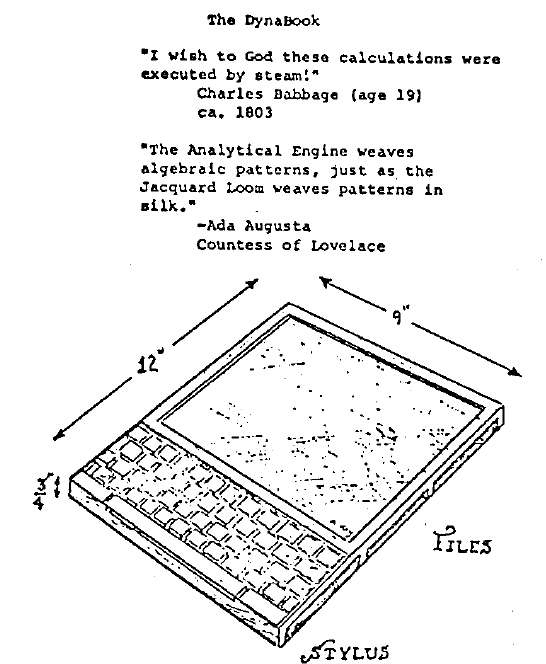
\includegraphics{images/original-dynabook-diagram-large.png}}} &
{\scalebox{0.5}{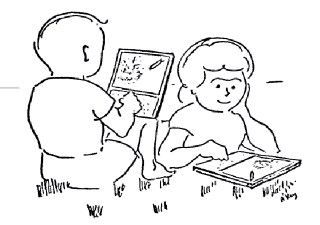
\includegraphics{images/dynabook-kids.png}} \vspace*{2ex}} 
\end{tabular}
\vspace*{1ex}
\bold{Dynabook Images}\\
{\small From Alan Kay, \emph{A Personal Computer for Children of All Ages}, 1972.}
\end{minipage}

\end{schemeregion}

